\chapter{Introduzione sulla Crittografia}
\section{Cifratura}
Quando vogliamo cifrare il contenuto di un messaggio in chiaro (\emph{plaintext}) abbiamo bisogno di un cifratore che sia in grado di trasformare il messaggio in un messaggio cifrato (\emph{cyphertext}) e un secondo cifratore in grado di decriptare il messaggio in modo tale da ottenere nuovamente un testo leggibile dal ricevitore. 
\begin{figure}[h]
    \centering
    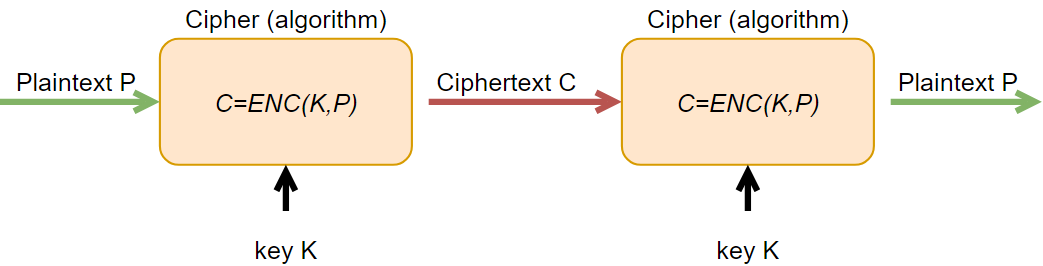
\includegraphics[width=\textwidth]{image/enc_exemple.png}
    \caption{Schema di Crittografia Standard}
    \label{fig:enc_exemple}
\end{figure}\\
La cifratura è una tecnica che serve \textbf{proteggere la confidenzialità dei dati} trasformandoli in qualcosa di incomprensibile ad un interprete generico. Come indicato nella \cref{fig:enc_exemple}, \textbf{la trasformazione} messa in atto da un cifratore \textbf{deve essere reversibile}, in modo tale che il destinatario del messaggio cifrato sappia ritrasformare il testo cifrato per poterlo leggere. Al fine di fare ciò, entrambe le parti devono conoscere due fattori:
\begin{enumerate}
    \item \textbf{Chiave:} la chiave è l'informazione che \textbf{deve} essere segreta e condivisa solo ed esclusivamente tra il mittente e il destinatario. Può essere di tipo \textbf{simmetrico} se viene usata la stessa chiave per cifrare e decifrare il messaggio, \textbf{asimmetrica} altrimenti. 
    \item \textbf{Algoritmo di Cifratura:} il meccanismo che applica la trasformazione al plaintext sulla base della chiave che viene segreta. Tipicamente gli algoritmi sono pubblici e standardizzati. 
\end{enumerate}
\subsection{Tecniche di Cifratura}
\begin{proposition}[Substitution Cypher]
Tecnica di cifratura che opera per sostituzione di lettere secondo un preciso schema (es: $A\rightarrow{B}$).
\end{proposition}
Il problema di sostituire secondo uno schema, detto dizionario, è che con un'analisi più o meno attenta (\emph{ad esempio analizzando la frequenza di ripetizione delle lettere}) è possibile dedurre lo schema di sostituzione e ricostruire il messaggio originale senza la chiave che era stata usata per cifrarlo. 
\begin{proposition}[Vernam Cypher]\label{prop:vernam}
Tecnica di cifratura che, dato un messaggio di lunghezza $L$, usa una chiave \textbf{randomica}\footnotemark di lunghezza $\hat{L}=L$ che vengono unite tramite $\oplus$ (xor) per generare il messaggio cifrato. Infine, sempre tramite $\oplus$, il messaggio viene decifrato usando la stessa chiave.
\footnotetext{La chiave deve essere generata in modo \textbf{truly random} ossia veramente casuale. Impossibile da fare tramite funzioni semplici, che generano sequenze di numeri pseudo-random.}
\end{proposition}
\begin{property}[XOR]
Ricordiamo che: $A\oplus{0} = A,\,A\oplus{1} = A',\, A\oplus{A'} = 1$.
\end{property}
Il vernam cypher è considerato il meccanismo di cifratura \emph{perfetto} in quanto se le ipotesi su cui si basa sono soddisfatto, il messaggio ottenuto in uscita è indecifrabile senza l'opportuna chiave. Tuttavia non è realizzabile, per i seguenti motivi:
\begin{enumerate}
    \item \textbf{Una chiave per ogni messaggio:} La robustezza del cifratore si basa sull'utilizzo di una chiave, completamente randomica, per ogni messaggio che viene inviato. Supponiamo di usare la stessa chiave $K$ per due messaggi cifrati $C_1$ e $C_2$ e facciamone lo $\oplus$:
    \begin{center}
    \vspace{-25pt}
        \begin{equation*}
            C_1\oplus{C_2}=(M_1\oplus{K})\oplus(M_2\oplus{K})=M_1\oplus{M_2}
        \end{equation*}
    \end{center}
    In questo modo abbiamo dedotto l contenuto del messaggio cifrato senza neanche sapere la chiave. Noto questo, tramite un \emph{Chosen Plaintext Attack} (attacco tramite invio di messaggi scelti), potremmo dedurre anche la chiave. 
    \item \textbf{Ogni chiave deve essere lunga quanto il messaggio:} Non un reale problema computazionale. Per rendere la chiave lunga quanto il messaggio, possiamo ripetere i caratteri della chiave se sono troppo pochi o usare metodi più sofisticati. Tuttavia scomodo dal punto di vista della scalabilità. Per $1GB$ di messaggio dovremmo disporre una chiave di $1GB$.
    \item \textbf{La chiave deve essere truly random:} impossibile da generare con funzioni di libreria o tecniche particolari, in quanto il numero casuale è definito da un algoritmo e, pertanto, generabile da terzi.
\end{enumerate}
\begin{corollary}[Lo scopo della crittografia]
Quando criptiamo un messaggio dobbiamo ragionare in ottica di \textbf{mettersi in sicurezza da una minaccia specifica}, piuttosto che da un pericolo in generale.
\end{corollary}\pagebreak
\section{Confidentiality, Integrity, Availability}
I principi alla base della cifratura e della crittografia sono i seguenti:
\begin{definition}[Confidentiality]\label{def:confidentiality}
Misura adottata per evitare che le informazioni sensibili arrivino alle persone sbagliate, assicurando che solo chi sia autorizzato possa accedervi.
\end{definition}
\begin{definition}[Integrity]\label{def:integrity}
Con il concetto di integrità si vuole specificare che, durante la trasmissione di un un messaggio, questo arrivi a destinazione \textbf{integro e senza che qualcuno possa alterarne il valore}
\end{definition}
\begin{definition}[Authenticated Encryption with Associated Data]\label{def:aead}
Un sistema in grado di garantire sia integrità che confidenzialità è detto di tipo AEAD.
\end{definition}
\begin{definition}[Availability]
Mantiene aggiornato e bug-free il software che veicola lo scambio del messaggio.
\end{definition}
Difatti, il modello di cifratura utilizzato fino ad ora non copre i casi in cui una minaccia intenta ad effettuare un attacco di tipo \emph{Man in the Middle (MITM)} riesca a modificare un bit o più del messaggio, modificandone il contenuto e passando inosservato. Possiamo dire che:
\begin{proposition}
Una cifratura mantiene un'\textbf{elevata confidenzialità} ma una \textbf{scarsa integrità}.
\end{proposition}
\begin{example}[ RFID:]
E' un sistema composto, solitamente, da un \emph{TAG} e un \emph{READER} (per esempio la carta e il pos). Per il funzionamento è necessario che tra i due oggetti ci sia una mutua autenticazione in quanto sia il \emph{TAG} che il \emph{READER} potrebbero non essere autentici.\\
Tipicamente un \emph{TAG} è composto da:
\begin{itemize}
    \item Un segreto, statico, $S$
    \item Una chiave, temporanea, $K$
\end{itemize}
Il messaggio contenente il segreto viene cifrato tramite $\oplus$ con la chiave associata all'utente.\\
Il \emph{READER} invece detiene un database con le chiavi degli utenti a cui fare riferimento.\\
Quando il \emph{TAG} viene a contatto con il \emph{READER}, quest'ultimo sarà in grado di decifrare il messaggio qualora fosse genuino, trovando un riscontro con qualche entry del database.\\
In questo sistema, ogni chiave è generata \textbf{pseudo-randomicamente} a partire dalla chiave precedente. Una volta ottenuto il segreto, il \emph{READER} associa una nuova chiave temporanea al \emph{TAG} in questione, aggiornando il suo database.\\\pagebreak
\begin{remark}
In un \emph{RFID} il segreto viene criptato usando una \emph{pseudo-random key}.
\end{remark}
Tale sistema presenta due problemi. Supponiamo che $S$ sia truly random e $K$ pseudo-random, allora:
\begin{itemize}
    \item Se $S$ è il plain-text, andando in \emph{xor} con $K$ \textcolor{red}{\textbf{viola la proprietà 3}} dei cifratori, in quanto la chiave non è truly random.
    \item Se $K$ è il plain-text, $S$ fa da chiave, ma \textcolor{red}{\textbf{viene violata la proprietà 1}}, in quanto la stessa chiave è associata a messaggi differenti.
\end{itemize}
Poiché l'algoritmo pseudo-random per generare la chiave è noto, è possibile dedurre tutte le possibili combinazioni di bit che costituiscono $K$. Pertanto, facendo uno \emph{xor} tra due messaggi consecutivi, è possibile ottenere un testo con cui fare \emph{xor} con una delle due chiavi, ottenendo delle combinazioni possibili per il plain-text originale.\\
Dato che $M_1\oplus{M_2}=7$, supponendo che $K_i=3,\,k_{i+1}=4$, confrontando con la mappa delle chiavi pseudo-random è possibile dedurre sia chiave, che messaggi che lo schema con cui vengono generate le chiavi.
\begin{figure}[h]
    \centering
    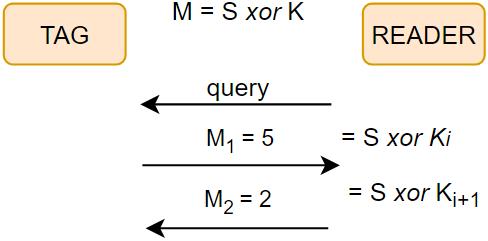
\includegraphics[width=0.6\textwidth]{image/rfid_example.png}
    \caption{Esempio di scambio messaggi in RFID}
    \label{fig:rfid_example}
\end{figure}

\end{example}\pagebreak
\section{Indistinguishability under Chosen Plaintext Attack}
Definire un \emph{"cifratore sicuro"} è generalmente difficile, in quanto una buona definizione deve tenere in considerazione la minaccia rispetto alla quale è considerato sicuro. Tipicamente viene adottata infatti la convenzione \textit{\textbf{Goal-Model}}.\\
Poiché un tipo di attacco è il cosiddetto \textbf{\textit{Chosen Plaintext Attack} (CPA)} una definizione che possiamo dare è che sia di tipo \textbf{IND-CPA}, ovvero, non deve rilasciare informazioni ad un'entità malevola quando questa possa attaccare il sistema sfruttando un plaintext scelto. Facciamo un esempio:
\begin{enumerate}
    \item Supponiamo che un attaccante \textit{A} abbia a disposizione due messaggi $M_0,M_1$ della stessa dimensione, che invia \textbf{in chiaro} ad un utente.
    \item L'utente sceglie randomicamente uno dei due, rispondendo ad \textit{A} con un messaggio cifrato: $C=ENC(K,M_0/M_1)$
    \begin{itemize}
        \item L'attaccante ha il $50\%$ di probabilità di ricevere uno dei due messaggi.
    \end{itemize}
    \item Supponiamo di avere a disposizione un \textbf{Oracolo}, in grado di conoscere \textit{l'associazione \textbf{chiave-testo cifrato}}. L'attaccante invia $M_0,M_1$ all'oracolo, che conoscendo $K$ può rispondere con $C_0=ENC(K,M_0),C_1=ENC(K,M_1)$.
    \item A questo punto l'attaccante confrontando le risposte ricevute, può individuare la chiave con cui viene eseguita la cifratura, con la stessa probabilità dei messaggi spediti all'utente.
\end{enumerate}
\begin{remark}
La chiave rappresenta un fattore fondamentale per garantire la confidenzialità, per questo sarebbe ideale avere a disposizione una chiave diversa ogni volta. In questo modo un attaccante non avrebbe possibilità di capire quale messaggio cifrato corrisponde ai suoi plaintext perché ogni volta riceverebbe un messaggio diverso.
\end{remark}
Le proprietà di un sistema dotato di \textit{"Indistiguishability"} sono:
\begin{itemize}
    \item Un avversario non deve essere in grado di ricavare alcuna informazione su un plain text a partire dal cipher text, anche se egli può avere accesso ad un oracolo.  
    \item L’encryption deve essere randomizzata, poiché uno stesso messaggio deve sempre essere criptato in diversi cipher text, che deve essere indistinguibile da uno randomico. 
    \item Se la sequenza si ripete essa deve essere criptata con una chiave differente
\end{itemize}
\begin{corollary}[XOR e Segretezza]
Dato il funzionamento dell'operatore $\oplus$, se cifriamo una sequenza di bit informativi con una sequenza di bit perfettamente randomica, possiamo dire con certezza che la sequenza generata in uscita sarà ancora casuale al 100\%. La probabilità di indovinare il plaintext a partire da quello cifrato è, a priori, quella di indovinare un numero casuale. Che sarebbe la stessa senza aver visto alcun cipher-text.
\end{corollary}
